\documentclass[a4paper]{article}
%\usepackage{exercise}

\renewcommand{\title}{Aufgabenseminar\\ Magnetismus}
\newcommand{\titleh}{Aufgabenseminar Magnetismus}

\usepackage{exercise} 
\usepackage{../images/preamble}
\usepackage{rotating}
\usetikzlibrary{decorations.pathmorphing}
\usetikzlibrary{decorations.markings}
\usetikzlibrary{arrows}
\usetikzlibrary{shapes.geometric}
\usepackage{mathrsfs}
\newcommand{\midarrow}{\tikz \draw[-triangle 90] (0,0) -- +(.02,0);}
\usepackage{xcolor}
%\usepackage{draftwatermark}
%\SetWatermarkText{\textsc{Entwurf}}
%\SetWatermarkScale{6}
%\SetWatermarkColor{red!30}

 
\fancyhead[L]{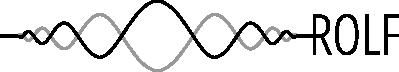
\includegraphics[width=2cm]{../images/logo_scaled.pdf}}
\fancyhead[R]{\textsc{\titleh}}



\begin{document}
	\vspace*{-1cm}
	\parbox{4cm}{\vspace{-0.2cm}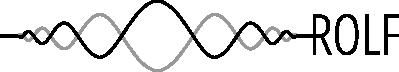
\includegraphics[width=5cm]{../images/logo_scaled.pdf}}
	\parbox{10.6cm}{\setstretch{2.0} \centering{ \huge \textsf{\title
			}}\\\url{pankratius.github.io/rolf}
			 }
		\vspace{0.5cm}
	
	


\noindent


\begin{Exercise}[difficulty = 3, origin = Estnisch-Finnische Physikolympiade 2014, title = Kraft zwischen Magneten, label = hangingmagnet]
	Um die Kraft zwischen zwei kleinen Stabmagneten zu finden, wird folgendes Experiment durchgeführt:\\
	Einer der beiden Magneten wird mit einem (masselosen) Faden der Länge $\ell = 1~\mathrm{m}$ an der Decke befestigt.\\
	Der zweite wird langsam an den ersten geführt, sodass die horizontalen Symmetrieachsen der beiden Magneten immer auf einer Gerade liegen.\\
	Als die Distanz der beiden Magneten gerade $4~\mathrm{cm}$ beträgt, hat sich der hängende Magnet $1~\mathrm{cm}$ bewegt. In diesem Moment verbinden sich die beiden Magneten schlagartig zueinander.\\
	Es kann angenommen werden, dass die Kraft $\vec{F}_m$ zwischen den beiden Magneten in der Form $|\vec{F}_m|\propto d^{-n}$ modelliert werden kann, wobei $d$ der Abstand der beiden Magneten ist, und $n\in \mathbb{N}$.\\
	Wie groß ist $n$?
\end{Exercise}
\begin{Exercise}[label = magneticpendulum, origin = {3. Runde zur 42. IPhO 2011}, title = Geladene Kugel am Faden, difficulty = 2]
	Eine geladene, kleine Kugel der Masse $m = 10~\mathrm{g}$ hängt an einme isolierenden, masselosen Faden der Länge $\ell = 1~\mathrm{m}$ von einer Decke herab.\\
	Sie befindet sich in einem homogenen, senkrechten Magnetfeld der Feldstärke $B = 50~\mathrm{mT}$. Die Kugel wird so in eine horizontale Rotation versetzt, dass der Faden einen Winkel von $\alpha = 30^\circ$ mit der Vertikalen einschließt.\\
	Die Rotationsfrequenzen im bzw. gegen den Uhrzeigersinn unterscheiden sich um $\Delta f = 2.0~\cdot 10^{-3}~\mathrm{Hz}$.
	\Question Wie groß ist die Ladung $Q$ der Kugel.
	\Question Wie groß ist der Mittel $\overline{f}$ der Rotationsfrequenzen?
\end{Exercise}

\end{document}
